%\documentclass[letterpaper, 12 pt, conference]{ieeeconf}  % Comment this line out
                                                          % if you need a4paper
\documentclass[a4paper, 10pt, conference]{ieeeconf}      % Use this line for a4
                                                          % paper

\IEEEoverridecommandlockouts                              % This command is only
                                                          % needed if you want to
                                                          % use the \thanks command
\overrideIEEEmargins
% See the \addtolength command later in the file to balance the column lengths
% on the last page of the document

% This is needed to prevent the style file preventing citations from linking to 
% the bibliography
\makeatletter
\let\NAT@parse\undefined
\makeatother

\usepackage[dvipsnames]{xcolor}
\usepackage{footmisc}
\newcommand*\linkcolours{ForestGreen}
\usepackage[dvipsnames]{xcolor}
\usepackage{scrextend}
\usepackage{times}
\usepackage{textcomp}
\usepackage{graphicx}
\usepackage{geometry}
\usepackage{amssymb}
\usepackage{gensymb}
\usepackage{amsmath}
\usepackage{breakurl}
\def\UrlBreaks{\do\/\do-}
\usepackage[breaklinks,pagebackref,colorlinks=false,
linkcolor=black,
filecolor=orange,      
urlcolor=brown]{url,hyperref}
%\usepackage{url,hyperref}
\hypersetup{
colorlinks,
linkcolor=\linkcolours,
citecolor=\linkcolours,
filecolor=\linkcolours,
urlcolor=\linkcolours}

%\usepackage{algorithm}
\usepackage{algorithmic}
\usepackage[linesnumbered,ruled,vlined]{algorithm2e}
\usepackage{algcompatible,lipsum}
\usepackage{caption}
\usepackage[labelfont={bf},font=small]{caption}
\usepackage[none]{hyphenat}

\usepackage{mathtools, cuted}

\usepackage[noadjust, nobreak]{cite}
\def\citepunct{,\,} % Style file defaults to listing references separately

\usepackage{tabularx}
\usepackage{amsmath}

\usepackage{float}

\usepackage{pifont}% http://ctan.org/pkg/pifont
\newcommand{\cmark}{\ding{51}}%
\newcommand{\xmark}{\ding{55}}%

\newcommand*\diff{\mathop{}\!\mathrm{d}}
\newcommand*\Diff[1]{\mathop{}\!\mathrm{d^#1}}
\newcommand*\imgres{600}


\newcolumntype{Y}{>{\centering\arraybackslash}X}

%\usepackage{parskip}

\usepackage[]{placeins}

% \usepackage{epstopdf}
% \epstopdfDeclareGraphicsRule{.tif}{png}{.png}{convert #1 \OutputFile}
% \AppendGraphicsExtensions{.tif}

\newcommand\extraspace{3pt}

\usepackage{placeins}

\usepackage{tikz}
\newcommand*\circled[1]{\tikz[baseline=(char.base)]{
            \node[shape=circle,draw,inner sep=0.8pt] (char) {#1};}}
            
\usepackage[framemethod=tikz]{mdframed}

\usepackage{afterpage}
\usepackage{stfloats}

\usepackage{atbegshi}
\newcommand{\handlethispage}{}
\newcommand{\discardpagesfromhere}{\let\handlethispage\AtBeginShipoutDiscard}
\newcommand{\keeppagesfromhere}{\let\handlethispage\relax}
\AtBeginShipout{\handlethispage}
\usepackage[export]{adjustbox} % loads also graphicx
\usepackage{comment}

\title{ \bf SASSCAL WebSAPI: A Web Scraping Application Programming Interface to Support Access to    SASSCAL's Weather Data
}

\author{Tsaone Swaabow Thapelo$^{*1}$,  Molaletsa Namoshe$^{2}$,  Oduetse Matsebe$^3$,\\
Tshiamo Motshegwa$^4$, Mary-Jane Morongwa Bopape$^5$  \\
%Department of Mechanical, Energy and Industrial Engineering$^{1,3,5}$\\
	%Department of Mechanical, Energy, and Industrial Engineering $^{1,2,3}$\\
	Botswana International University of Science and Technology (BIUST)$^{1,2,3}$\\
	%	Department of Computer Science, 
		University of Botswana$^4$\\
			South African Weather Services, Pretoria, South Africa$^{5}$ \\
		{*\color{black}Corresponding Author}: {\color{black}swaabow@gmail.com}
}



\setlength{\columnsep}{1cm}
\newgeometry{layoutwidth  = 8.2500in,
	layoutheight = 11.20in,
	vmargin      = 00.50in, %Inches at top
	hmargin      = 00.60in,
	headheight   = 00.50in,
	headsep      = 00.15in,
	footskip     = 00.60in}
\pdfpagewidth  = 8.2500in
\pdfpageheight = 12.00in

\begin{document}

\maketitle
\thispagestyle{empty}
\pagestyle{empty}


%%%%%%%%%%%%%%%%%%%%%%%%%%%%%%%%%%%%%%%%%%%%%%%%%%%%%%%%%%%%%%%%%%%%%%%%%%%%%%%%
\begin{abstract}
\noindent
The Southern African Science Service Centre for Climate and Land Management (SASSCAL)  was initiated to support regional weather monitoring and climate research  in Southern Africa.
As a result, several Automatic Weather Stations (AWSs) were implemented to provide numerical weather data within the collaborating countries. 
%Problem
 Meanwhile, access to the SASSCAL weather data is limited to a number of records that are achieved via a series of clicks. 
 Currently, end users can  not efficaciously extract the desired weather values. 
Thus, the data is not fully utilised by end users. % like students, researchers, contractors and local meteorologists. 
 % one sentence about research/study objective,
 This work  contributes with an open source Web Scraping Application Programming Interface (WebSAPI) through an interactive dashboard. 
 The objective is to extend functionalities of the SASSCAL Weathernet for: data extraction, statistical data analysis and visualisation. %generating data sets that is ingestible to data mining workbenches for further statistical analyses. 
 %Methods
  The SASSCAL WebSAPI    was developed using the R statistical environment. 
  It deploys  web scraping and data wrangling techniques to support access to SASSCAL weather data. % and  ultimately generate .  
 %Results
% The generated tables and figures can be exported as .csv or .pdf files. %A hypothetical dataset was used to demonstrate the application of the SASSCAL WebSAPI.
 %conclusion
 This WebSAPI reduces the risk of human error, and the researcher's effort of generating desired data sets.  %The overall gain is the  efficacious use of the data collected by the  AWSs maintained through the SASSCAL initiative. 
  % a sentence about the significance of that finding.
  The proposed framework for the SASSCAL WebSAPI can  be modified for other weather data banks   while taking into consideration the legality and ethics of the toolkit.  %
\\
\\
\emph{Key Words}:   Data Access, Data Analysis, Data Visualisation
\end{abstract}

%%%%%%%%%%%%%%%%%%%%%%%%%%%%%%%%%%%%%%%%%%%%%%%%%%%%%%%%%%%%%%%%%%%%%%%%%%%%%%%%
\section{\textbf{Introduction}}
\label{Intro}
\noindent
Meteorological weather   data are useful 
in filling information needs in  academia and industrial settings.  The   information generated from these data at local levels is  useful in complementing:  hydrological models \cite{schuol2007using}, high impact weather predictions models \cite{chang2013international}, and simulations of heavy rainfall events \cite{molongwane2020sensitivity,somses2020convection,bopape2021sensitivity} and heatwaves \cite{moses2017heat}. 
Moreover, weather data are also vital for agro-meteorological operations, as well as in efficacious planning of construction and recreational activities. 
Although there is a huge need of weather or climatological  data for Southern Africa, various institutions and   enterprises   like BIUST, SASSCAL\footnote{\url{https://www.sasscal.org/}\label{SASSCALQ}}  and WASCAL\footnote{\url{https://wascal.org/}\label{Wascalnet}}    have  introduced  AWSs to monitor weather events at finer   intervals. \\

However, most of  AWSs installed in developing countries are underutilized.   For instance, the Botswana Department of Meteorological Services (BDMS)'s mandate is to provide quality weather, climate information and services to enable informed decision making for sustainable socio-economic development in scenarios related to weather and climate. %The BDMS also provides guidance on building resilience to climate change. 
Meanwhile, the  BDMS lacks a designated online platform (currently relies on    radio stations, television and a Facebook page)    to disseminate  weather information  to the public.

\newpage
\noindent
 %The current BIUST system is maintained by the Sutron Company based in USA. This makes it intricate for local technicians or developers to integrate new services  for collection and dissemination of weather data.  
   On a related note,  BIUST identified ``Climate and Society" as one of its   \emph{thematic areas}\footnote{\url{www.biust.ac.bw/research/thematic-areas-platforms/}\label{biust}}  of focus. This  is geared towards enhancing services related to:  climate and impact modeling; early warning, and  disaster     management for weather and climate change.
In 2016, BIUST installed  an AWS equipped with a local machine running XConnect %\footnote{\url{www.sutron.com/product/xconnect-software/}} 
for data logging of historical weather data.
    Likewise, this particular AWS also lacks the backend service layer for dissemination of weather outputs to end users. All these can be seen as  barriers and hence limitations of access to the generated weather data.
For instance, to request data, clients have to go through some hectic   processes. In the case of BIUST, clients have to request data using email, or copy it from the officers using physical storage devices like memory cards. In case of BDMS, end users  download and complete a form\footnote{\url{https://www.gov.bw/natural-resources/request-climatological-data}\label{Formo}};  then submit it to   BDMS. The service time is three    days long.\\
  
It is irrefutable that, the  demand of climatological data in Southern Africa %in order to assess recurrent climatic extremes and its implication for natural and human systems, this work finds its necessary for
 invites key stake holders (i.e., researchers and developers) and organisations to implement platforms that facilitate ease access and visualisation of climate data.
 %for the analysis of weather extremes.
As a result, the Southern African Science Service Centre
for Climate and Land Management (SASSCAL) was
initiated \cite{helmschrot2015sasscal} to support regional weather monitoring and climate
research in Southern Africa \cite{muche2018sasscal}. The SASSCAL Weathernet\footnote{\url{http://www.sasscalWeathernet.org/}\label{Weatherneto}} % (seeFig \ref{SASSCA}) 
disseminates near to real-time  data  from AWSs at    hourly intervals, including aggregated daily and monthly  data. 
%The collected data (i.e., since 2014 in Botswana)  include: temperatures, solar radiation, relative humidity, rainfall and sunshine duration, among others. Such   data is vital in environmental data science \cite{GIBERT20183}.

\begin{figure}[tbh!]
\centering
\includegraphics[width=1\columnwidth]{fig/SasscalWeathernet.png}
\caption{Visualisation of   AWS   data via the SASSCAL Weathernet  \ref{Weatherneto}.}
\label{SASSCA}
\end{figure}

\newpage
\noindent
	The SASSCAL weather  data is  reviewed for quality control   before dissemination  \cite{kaspar2015sasscal}. These data can also be integrated with
data from different sources for research purposes. For
instance, Moses et. al. \cite{moses2018effects} merged it  with
other meteorological data from the BDMS to analyse effects of solar radiation,
wind speed and humidity on evapo-transpiration around
the Okavango Delta. Similarly, predictive data analysis and modeling of   temperature
patterns   \cite{thapelo2019machine,thapelo2014tecnicas} is vital in the understanding of heatwaves \cite{moses2017heat}; while
rainfall values can help in assessing rainfall erosivity \cite{singh2020assessing}.
%   	   \newpage
\\
\\
\noindent
Despite the distinct potential use of the SASSCAL weather data, there is a burden on the end users to access, download and use such data in research (see Fig. \ref{datamunging}). % Currently, users can only
	%The current access mechanisms deployed by the SASSCAL Weathernet \ref{Weathernet} only allow end users to
%Currently, end users can 	view weather data and manually download  subsets of data at a time following steps in Fig. \ref{datamunging}. % using a set of clicks. % (see Fig. \ref{datamunging}).
	First, the user has to navigate to the SASSCAL Weathernet to identify a country,   AWS  of interest, and the temporal resolution of the   weather data. % (hourly, daily or monthly).
The user can then manually copy and paste the whole data to a storage file for data analysis. There is an option to download the SASSCAL weather data in excel format only. %(currently not working). % as seen in Fig. \ref{BugUno}).
	%Even when this option is working, the steps of downloading the data are not obvious to new users. 
	However, there is no option to only select the desired weather values from AWSs of interest. Even after downloading the weather data, end users face a challenge of generating clean data sets containing the desired variables for further use. 
   	    The situation worsens when extracting finer  temporal data   from multiple AWSs across the  entire region. 
	%All these challenges  	limit the 	effective 	use of these weather data in specific  projects.
	\begin{figure}[h]
   		\centering
   		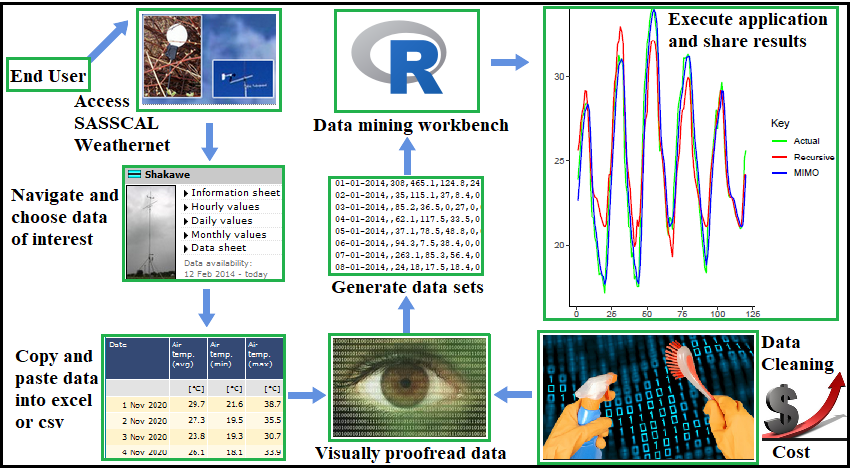
\includegraphics[width=0.98\linewidth]{fig/MiPipe}
   		\caption{Manually extracting data  from the  SASSCAL Weathernet. This process is costly, time consuming and error-prone. }
   		\label{datamunging}
   	\end{figure}
   	
 \noindent
This work presents the SASSCAL Web Scraping Application Programming Interface (WebSAPI).  
%AWSs provide numerical weather data that has potential to catalyse the development of robust responses to climate related problems. 
   	    % in their projects. %  All these invite techniques of data science. %web scraping, data wrangling and dashboard applications 
   	 %to extend the functionalities of the SASSCAL Weathernet. % to serve  users.
  % 	 \newpage
   %	 \noindent
  % 	 %	However, extraction of  the desired SASSCAL weather  data by end users  is not efficacious as discussed in section \ref{Intro}. 
%	
%		\begin{figure}[h]
  % 		\centering
  % 		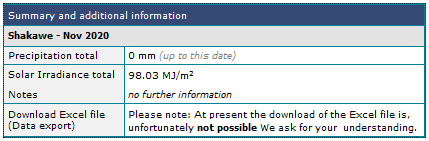
\includegraphics[width=1\linewidth]{fig/BugUno}
  % 		\caption{The SASSCAL download option currently not working}
  %% 		\label{BugUno}
 %  	\end{figure}
%	
%	\noindent
%	Currently, there are no web scrapers in existence to support efficacious access to the SASSCAL  weather data. 
	%To address this gap, this work deploys the basic concepts of web scraping in \cite{yang2010development,glez2014web,BONIFACIO201513,bradley2019web} to develop the SASSCAL WebSAPI  for  visualisation and downloading of  consecutive SASSCAL  weather data of interest. 
	% These limit the use of the SASSCAL data in research. \\
%	 \\
%\\
%\\
Web scraping \cite{WebSrapping} is a data science technique that deploys scripts for extraction  of structured data from websites. % to meet end users' requests.
 A script is a computer program that automates a specific task using some selected programming languages like R or Python. 
 Thus, a WebSAPI can be seen as an application service that allows access to online data for further use in research projects. 	 
By digitalising the  BDMS' form in \ref{Formo} for climate data requests, this work will be enabling end users to efficaciously (1) access and visualise weather data from the   SASSCAL Weathernet; and (2) download desired data  for  use in  data driven  projects.   % In particular, the work uses Botswana and Shakawe as case studies.
\\
\\
The structure of the work is as follows. Section \ref{LR} provides a   brief background information to   this work. Section \ref{Mtods} presents the   approach deployed in the development of the SASSCAL WebSAPI. % and its basic functionalities. 
   Section \ref{Res} presents results. It also illustrates how the SASSCAL WebSAPI can be used to support the extraction of weather variables, as well as the visualisation and dissemination of the generated outputs. %around the Okavango Delta. %as an example of the benefits of having supportd tools for web scrapping tools. 
Lastly, section \ref{Discus} and  \ref{Conclu} present discussions and conclusions. % respectively.
%including the implications and limitations of the SASSCAL WebSAPI. 
   %Section \ref{Conclu} presents   conclusions and future from this work. % resulting from this work.

\section{\textbf{Related Literature Review}}
\label{LR}
\noindent
%The huge demand of climatological data in Southern Africa  invites  collaboration of key stake holders like researchers, developers, and decision makers. 
%Climate informatics \cite{lyubchich2019statistics,GIBERT20183} is a new multi-disciplinary field that integrates statistical machine learning,  climate science, data science, application development as well as   mechatronics and  instrumentation  to bridge the gap between weather services and   end users.
Most of African countries \cite{dinku2014bridging}  like Botswana \cite{Nkemelang2018} are lagged behind  in terms of climate informatics \cite{lyubchich2019statistics} and environmental data science \cite{lyubchich2019statistics,GIBERT20183}.  
This can be attributed to lack of readily available platforms and   data as also pointed out  in   \cite{schuol2007using,dinku2014bridging}. All these bottlenecks can be unlocked by integrating computing technologies like web scraping and dashboard applications. Web scraping techniques have been widely deployed in a number of projects from different disciplines such as economics \cite{smith2020making} and climate science \cite{yang2010development}. \\
\\
Regardless of the discipline, the general idea is to allow greater visibility, access, extraction and usability of the online data.  
This work contributes by addressing the second ``pillar" of the Global Framework for Climate Services \cite{VAUGHAN201665} using climate informatics.
This WebSAPI is motivated by authors in  \cite{BONIFACIO201513} who presented a free tool for automated extraction and consolidation of climate data from different online web data banks.   A similar work by Yang \emph{et. al.} \cite{yang2010development} presented a system with functionalities for scraping, filtering and visualising climatic data for easy use.   This work is related to Ref \cite{sitterson2020demonstration} regarding the user API for data request.
 	It is also related to \cite{BONIFACIO201513} in such it deconstructs the URL for a given station and then modifies the date range and the desired temporal resolution to extract desired weather data. 
\\
\\
Web scraping is still   emerging, with no dominant standards at current.  This technology also presents a combination of   ethical and legal challenges \cite{mason1986four,krotov2020tutorial} that necessitates  standards   to support data exchange. The ethical issues       attached to web scraping can be summed into four generic groups: \emph{property}, \emph{privacy}, \emph{accessibility} and  \emph{accuracy}  \cite{mason1986four}.
\begin{enumerate}
    \item The  \emph{property} aspect of it entails ownership of data and its possible use. % (i.e., Intellectual Property rights).
    In this context,  a web scraping algorithm (WSA)  can lead to infringement of copyrights, especially  when end users make profit out of the  data without the consent of data owners \cite{dreyer2013internet}.
    \item Regarding \emph{privacy},  web scraping can unintentionally reveal  details or  flaws within an organization \cite{mason1986four}. For instance, a web scrapper can reveal data structures as well as some sensitive data hidden from end users \cite{ives2006anything}. 
    %This can raise ethical issues with    development team of organisations.
    \item  In terms of \emph{accessibility} \cite{mason1986four}, it is noted that a WSA can overload a website, which may ultimately   cause damage to the organisation's  web server. Moreover, web scraping can result in unintended and un-predicted harmful consequences to   the website's server \cite{krotov2020tutorial}.  
    
    \item The \emph{accuracy} aspect of WSAs is mainly concerned with  the authenticity and fidelity of the generated data \cite{mason1986four}. This is crucial since erroneous data generated through a WSA may   mislead   end users or even damage the reputation of a particular organisation's  website.
\end{enumerate}
Web scrappers can  also compete with the main data provider APIs, % of a particular organization, 
which might diminish  the value of the organisation's intended mission
\cite{hirschey2014symbiotic}.  For instance, if a   web scrapper  attracts more clients than the  intended main API, then end users might end up neglecting the  platform of that   organisation.  %(i.e., SASSCAL) 
%although it provides more information. % in addition to the collected   data. 
All these invite multi-disciplinary collaboration  (i.e., government sectors, academia and industrial practitioners)  to establish 
  standards  and boundaries for technology usage. This could irrefutably catalyse the development and adoption of the generated data driven outputs as also supported in \cite{fundel2019promoting,katz2005economic}.
  \newpage
\section{\textbf{Methodology: Data, Tools and Methods}}
	\label{Mtods}
	\subsection{\textbf{Data Sources and the SASSCAL WebSAPI}}
\noindent
The first task was to identify the data sources, and the SASSCAL Weathernet came to the rescue.
	The aim of the SASSCAL WebSAPI is to improve data accessibility and visualisation of the SASSCAL Weather data before data analysis and predictive modeling. The  target of this work was to develop and implement independent algorithms that can, later on, be consolidated and integrated into a package for data driven projects requiring   SASSCAL weather data.
%Botswana is landlocked country in Africa. The country is situated between longitudes 20\textdegree E and 29\textdegree E, and between latitudes 17\textdegree S and 27\textdegree S. 
%The country has a hot and semi-arid to arid climate. The highest maximum air temperatures are observed between October and March  (summer period) \cite{moses2017heat,ARCHER201722} with mean monthly  temperatures ranging between 30.9\textcelsius\ and 33\textcelsius. These are normally accompanied by heat waves, with maximum temperatures going up to $\approx$42\textcelsius\ \cite{moses2017heat}. 
\\
\\
	The SASSCAL WebSAPI comprises of modularised algorithms packaged into scripts to enable direct control of  weather data provided by the SASSCAL weathernet. This include but not limited to algorithms targeted at: processing the SASSCAL Weathernet link;  determining the pages containing  relevant weather data;   deconstructing and parsing   contents of the \emph{HTML} file; extracting  required weather data from   selected pages;  combining    data (i.e., data wrangling) into   data frames to generate  data sets and visuals; as well as sharing the generated outputs   using interactive dashboards.
%\begin{figure}[h]
%	\centering
%	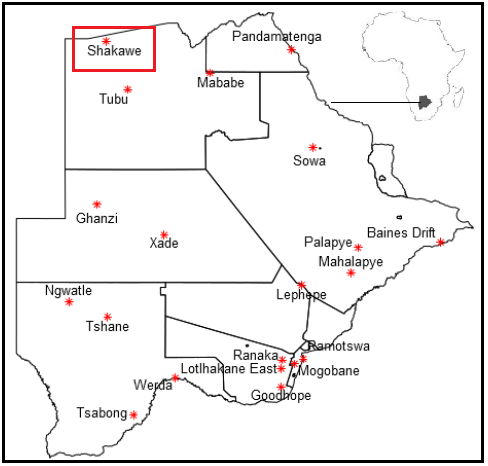
\includegraphics[width=1\columnwidth]{fig/Map20.png}
%	\caption{Data source area (Shakawe) in the North-West of Botswana.}
%	\label{Shakawe}
%\end{figure}

\subsection{\textbf{Analysis of the SASSCAL Weathernet}}
\noindent
The SASSCAL Weathernet   enables the public to use one domain to access the AWS data.
Each SASSCAL country member  has various AWSs,  each   with a unique   identifier (ID). 
Access to the      data  is defined using the same abstract pattern.
 In essence,  one can query the website’s database for any AWS within the SASSCAL region by providing the  corresponding URL.
 Thus, one can extract the weather data via a tailored API using formats like HTML and XML. 
%The SASSCAL Weathernet allows only URLs   pointing to the corresponding AWS data. 
\\
\\
 The  home page  $URL$ for each SASSCAL AWS data is	defined by: $x/y?z$; where
%	\begin{equation}
%		L = x/y?z.
%		\label{pattern}
%	\end{equation}	
%
%In Eq. \ref{pattern}, % $L$ is the complete $URL$ for the data of interest, 
$x$ is the preamble in link  \ref{Weatherneto};
$y$ is just the $weatherstat\_\alpha\_AO\_we.php$ token that defines the weather statistics for a given  resolution (monthly, daily or hourly); and $z$ is the string describing the logger ID ($loggerid\_crit=n$), where $n$ is the AWS' unique  ID.  Tables containing  relevant data   are found by trial and error (i.e., by   inspect individual elements of the SASSCAL weathernet page, or just exploring  the source code of the web page. % process.
%	The proposed  toolkit is equally applicable to AWSs within collaborating countries. 

\subsection{\textbf{Identification of Tools and Methods}}
\noindent
	This work deploys the workflow depicted in Fig. \ref{Flw} following the data science approach in \cite{wickham2016r,bradley2019web}  %to tailor the CRISP  as seen in  Fig. \ref{Flw}
 using open-source platforms (i.e., R version $4.0.3$ and RStudio $1.1.463$). 
 %R is simple to learn, and is supported by a large community of statisticians and developers. 
Thus, the algorithms are coded in R, and the functions are tested using the RMarkdown which facilitates  reproducibility.
 R   has  excellent packages for  statistical data science and visualisation. Table \ref{tabla} shows   packages deployed in this work.
% reactive maps, charts and tables. %    to visualise and    disseminate  outputs.  control over  data
%, including    reproducibility of the proposed approach.
%Although the deployed skill set are transferable to other SASSCAL country members. %, the scope of illustrations here is limited to Botswana, with some illustrations of weather extremes focused on      Shakawe AWS. 

\begin{table}[h!]
 \caption{R packages proposed in this work}
\centering
\begin{tabular}{||c | c||} 
 \hline
 Package &  Description    \\ [0.5ex] 
 \hline\hline
rvest  \cite{wickham2016package} & for web scraping   \\ \hline
 Xml2 \cite{lang2015package}   & for XML document processing  \\ \hline
   stringr \cite{wickham2019package} & for data cleaning and preparation tasks   \\ \hline
  ggplot \cite{wickham2011ggplot2} & for visualisation of graphics   \\ \hline
 shiny \cite{chang2015package} & for  dashboard design   \\ \hline
  leaflet  \cite{graul2016package} & for  reactive maps   \\ \hline
%		\caption{to retrieve the ID of a given  AWS}
dygraphs \cite{vanderkam2015dygraphs} & for  charting time-series data and interactivity   \\ \hline
%		\caption{to retrieve the ID of a given  AWS}
% raster   \cite{hijmans2015package} & to process   shape-files and visualise maps \\ \hline
% dplyr   \cite{wickham2015dplyr} &    A Grammar of Data Manipulation  \\ \hline
  data.table \cite{dowle2019package} &  for  tables and  data manipulation   \\ \hline
       flexdashboard \cite{allaire2017flexdashboard} &  for  flexible shiny dashboard   \\  %[1ex] 
 \hline
\end{tabular}
\label{tabla}
\end{table}
\newpage
\noindent
 A helper function (\emp{helper.R}) is scripted to install and load the packages included in Table \ref{tabla}.
The \emp{rvest} \cite{wickham2016package} package is required  for web scraping; while the XML \cite{lang2015package} is required for XML document processing. The   ggplot \cite{wickham2011ggplot2} is used for data visualisation. 
The  shiny \cite{chang2015package}   and Flexdashboard \cite{allaire2017flexdashboard} packages are used to design  the WebSAPI's  dashboard.
The \emph{htmlwidgets} framework is deployed to provide high-level R bindings to the JavaScript  libraries for data visualization.  All these functions are embedded in a reproducible RMarkdown  to implement the proposed SASSCAL WebSAPI.
The  data driven pipeline used in this work is summarised  in Fig. \ref{Flw}.
\begin{figure}[h]
		\centering
		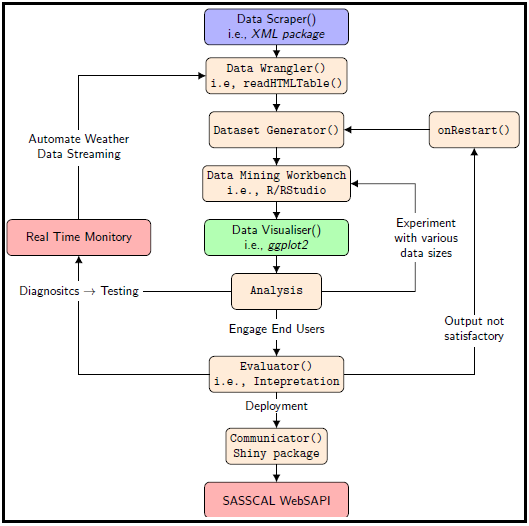
\includegraphics[width=1\linewidth]{fig/MiPipeLine}
		\caption{Workflow of the  SASSCAL WebSAPI}
		\label{Flw}
	\end{figure}
\noindent
%This work focuses on the utility of the dashboard API than on   data analysis of weather extremes. 
%The Data Fetcher  % based on the request from the Data Requester. 
%The Data Parser  
%The Data Wrangler  
%The  Communicator  %to visualise,  explore and download weather data. %the  weather data. %It serves as an interface between the end user and the data availed by the SASSCAL Weathernet. 
 %Packages used in this work include:    The raster   \cite{hijmans2015package} and  maptools  \cite{bivand2013maptools} packages were used to process   shape-files and visualise location based geographic data.
 %(see the Botswana map depicted in Fig \ref{BW}).
%dygraphs, which  and includes support for many  features including series/point highlighting, zooming, and panning.
 % in research and decision making purposes. 
\subsection{\textbf{Visualisation of AWSs using Interactive Maps}}
\noindent
Algorithm \ref{TheMapper}  implements an interactive map  to visualise  where the AWSs are located geographically. Here,  $w$ is a vector of AWSs for a given country, $x$ and $y$ are vectors of the latitude and longitude coordinates of the AWSs, $z$ is a vector detailing  the descriptions of a given AWS. The algorithm also allows  users to select specific AWSs; thanks to the \emph{leaflet}   package.

	\begin{algorithm}
		\caption{Visualise the AWSs of a given country}
		\label{TheMapper}
	%	\KwIn{w,x,y,z}
	%	\KwOut{Distribution of AWSs on a map}
			c$\leftarrow$dataframe($w,x,y,z$)\\
			%\tcc{Select the desired table}
			\emph{leaflet}(data = c) $\%>\%$ \\
		addTiles() \%$>$\% \\
  setMaxBounds($x_1,y_2, x_2, y_2$) \%$>$\%\\
  addMarkers(\sim long,\sim lat, label= \sim name)%

	\end{algorithm}
	
	\noindent
In Algorithm \ref{TheMapper}, the dataframe `\emp{c}' defining the inputs  is  piped into the 	\emph{leaflet} function    to automatically generate an auto-size map that fits markers of all  AWSs. This function also   adds some bounds in (Line 4) so that the user can’t scroll too far away from the  markers of AWSs. The interactive map pops up the name of the AWS as the user hovers the mouse over a marker.  This simple functionality is crucial for end users (i.e., researchers) since it provides spatio-visual  exploration  of AWSs that are supported by the SASSCAL weathernet.

\newpage

\subsection{\textbf{Web Scraping and  Dataset Generation}}
\label{Scraper}
\noindent
 The web scraping functionality  in Algorithm \ref{AWS_ID_Getter}  uses the \emph{All$\_$AWS$\_$ID.R} script to construct vectors and store  names and IDs of  AWSs.
  The \emph{AWS\_ID\_Getter} function  assigns an AWS name (i.e., ``x") to its corresponding ID (i.e., ``value") using a hash map function (see Line 7 and 8). 
Thus, to find the ID for a given AWS of interest, the function looks-it-up  into the hash function  and   retrieves the address of that AWS' ID. 
\begin{algorithm}
	\caption{Data scraper}
	\label{AWS_ID_Getter}
$AWS$\_$ID$\_$Getter$$\leftarrow$ function(AWS) \{\\
 V = c(``x", ``value"); parent = emptyenv()\\
  assign$\_$hash $\leftarrow$ Vectorize(assign, vectorize.args = V)\\
  get$\_$hash $\leftarrow$ Vectorize(get, vectorize.args = ``x")\\
  exists$\_$hash $\leftarrow$ Vectorize(exists, vectorize.args = ``x")\\
  source(``All$\_$AWS$\_$ID.R")\\
  hash $\leftarrow$ new.env(hash = TRUE, parent, size = 100L)\\
  assign$\_$hash(AWS$\_$Name, AWS$\_$ID, hash)  \\
  ID$\_$Getter$\leftarrow$hash[[AWS]] \\
  return(ID$\_$Getter)
\}
\end{algorithm}

\noindent
The AWS name, ID and date are then  used to construct a URL used to fetch the data by the \emph{DataHaverster.R} function in Algorithm  \ref{DH}. The \emph{DataHarveter} takes in a  $URL$ to a given AWS. The URL string can be partitioned into tokens (i.e., using just the AWS name and date) to facilitate easy input. % as discussed previously.
%As mentioned in the introduction section, this can overload the server. To avoid this, the URLs can be manually changed by the user using some mouse clicks. The data is then saved in a data frame ready for further exploration, and even predictive data analysis.
%\subsection{\textbf{Phase 5: Data Visualisation and Dissemination}}
%\noindent
%We visualise the sample output data from the SASSCAL WebSAPI search query using the designed dashboard.
%As one can see from the output in JSON format (see Appendix B), the API does not allow one to achieve actual AWS descriptions.  We opened one of these URLs in a browser for further analysis. Alternatively, one can use the “inspect” feature provided by the web browser to analyse the description of a platform's underlying code in order to determine which elements contain the needed AWS data. One can write a code to retrieve the actual AWS for each given date with the API using an R script.
%\noindent
 % extraction of the  SASSCAL weather data and the generation of   datasets.
%The  $read\_html()$ function    takes in as input the $URL$ of the targeted AWS to create a Document Object Model that will hold all the weather data and structure of the targeted SASSCAL web.  We then use the use the $html_nodes()$ function to extract tables of interest.  
%The \emph{Data Wrangler()} method  uses the \emph{dplyr} package \cite{wickham2015dplyr} to provide end users with the functionality of selecting the desired weather variables based on their names.  % The \emph{Dataset Generator()} function  generates consistent formats    for  analysis and modelling. % in goal of these tools is to enable web scraping, data wrangling,  and visualisation. 

\begin{algorithm}
	\caption{Data harvesting}
	\label{DH}
	$\mu$ $\leftarrow$ TheHarvester(AWS$\_$NAME,DATE,$\rho)\\
	$DOM$ $\leftarrow$ $readHTMLTable(URL)$\\
			$\mu$ $\leftarrow$ $DataWrangler($as.data.frame(DOM[\beta]))$ \\
	 datatable($\mu$, $\phi$, $\omega$)

\end{algorithm}

\noindent
 %The output is  for  generation of   weather data sets.  
 The  \emph{XML} package \cite{lang2013package}  was used  to parse a given \emph{URL} and create a Document Object Model ($DOM$). %  as seen in Algorithm \ref{WebScraper21}.
This \emph{XML} package uses the $readHTMLTable()$ function %which can be used 
to  specify the weather data to  select from  the HTML tables in the SASSCAL Weathernet. 
 The number of tables for a given $DOM$  was  determined using R's built-in  \emph{length()} function. There are three $DOM$ instances for each temporal resolution; each with  multiple tables. 
%Some tables contain non-numeric data and information like figures (see Fig. \ref{BugUno}).
%We  extract   tables with numerical values.
%A visual inspection of the SASSCAL Weathernet page reveals that there are several tables used to visualise data and  information. 
There are 14 tables in the $DOM$ corresponding to the web page with  hourly data, and the values of  interest are in the $13^{th}$ table. The $DOM$ for  the web page with   daily observations has   13 tables, and daily values of interest are in the $12^{th}$ table. The last $DOM$  has 18 tables with    monthly  data contained  in the $10^{th}$ table. 
\\
\\
Line 3 in algorithm \ref{DH}  facilitates the cleaning and selection of  desired weather tables  using the parameter $\beta$ (i.e., $\beta$ can be 13, 12 or 10 as discussed above). 
%To reduce the scope of articulations presented inhere, this work only retrieves the hourly data. 
The parameter $\phi$ defines the extensions to fix the columns of a table to be visualised; while $\omega$ defines extra options for buttons    to facilitate end users to search, scroll, copy and download the weather data visualised via the table.
 The  $DataWrangler()$ function was implemented to iterate through the table containing  dates of  observations. It uses the $\rho$ argument to determine the date range  for the data of interest. The extracted weather data is then unified into a single data frame $\mu$ to generate   data sets for further use as illustrated in Fig \ref{BW_Map} and 
  \ref{SASSCAL_WebSAPI} in section \ref{Res}.
  
\subsection{\textbf{Dashboard Design: The Graphical User Interface (GUI)}} 
\noindent
%The SASSCAL Weathernet portal in \ref{Weathernet} provides a Graphical User Interface (GUI) for dissemination of the climatic data to end users.  As mentioned in section \ref{Intro}, efficacious access to such data is not trivial since end users are required to use a series of clicks and can only download the desired  data using a number of clicks. %The following algorithm completes the download
Algorithm \ref{WebScraper} implements  functionalities for the dashboard page. This include the $dashboardHeader()$ to define the title; and   the $dashboardSidebar()$ to define  two functionalities of  visualising   the tables of numerical weather data from an  AWS of a given country. The $dashboardBody()$  facilitates selection of the AWS, the  resolution, date range, use of data,  and   weather values and the functionality to also export data. 
Since different end users have different user needs, this work does not develop a complete GUI. Interested readers should see Ref \cite{smith2020making} for completing a dashboard API.

%\subsection{\textbf{Phase 7: Testing the SASSCAL WebSAPI}}
%\noindent
%The first test involved the deployment of the developed WebSAPI to collect a moderate data set that comprised 19 observations.
%The query to the server was made using  Dell Laptop (Processor: Intel® Core™ i5-4590 CPU @ 2.50 GHz, RAM: 8GB, running Windows 10 Pro.)  to download daily AWS data in less than 30 seconds.
% It was concluded that such scraping rate would not likely   overload the SASSCAL Weathernet server  in a way that can affect it from providing related services to other clients.

\begin{algorithm}
	\caption{Dashboard design for dissemination}
	\label{WebScraper}
	\KwIn{It requires Algorithm \ref{WebScraper}.}
	\KwResult{SASSCAL WebSAPI GUI}
	\While{(Interactive)}
	{
		gui $\leftarrow$ fluidPage(
			{
		$F$ $\leftarrow$ DataScraper()   %\tr{Create a dataset $miFichero$ for modelling}
	}\\
		$T$\leftarrow$ dashboardHeader(...),\\
		$SDB$\leftarrow$ dashboardSidebar(...),\\
		$B$$\leftarrow$dashboardBody( fluidRow(...))
		)\;\\
		server $\leftarrow$ function(I,O) \{ Communicator($F$) %	X = Actual$\leftarrow$ tail(MAXTMP[(n-(LB)):n],h)\\
		\};\\
		shinyApp(gui, server)\;
}
\end{algorithm}

\section{\textbf{Results}}
 \label{Res}
\noindent
This work documents the development process of a  lightweight WebSAPI capable of extracting and  displaying  timely weather data based on the SASSCAL weathernet. The WebSAPI is cost-effective since it is powered by open source technologies. Besides  the  functionalities of extracting  numerical  data,   the WebSAPI's tasks were expanded
  to include visuals using other  formats like tables, maps, and charts. 
 Fig \ref{BW_Map} shows an interactive map generated using   Algorithm \ref{TheMapper}. The interactive map can pop-up the name of the AWS  as the user hovers the mouse over a marker.
  %illustrations on how the developed functionalities can be deployed to visualise graphs and tables to end users.
%Interpretation
%As a specific use case this tool may be of particular value for the challenging risk assessment and risk
%communication in the context of the Summer Olympic Games in Japan 2020 and similar situations
%elsewhere.
 %The data set used  contains daily %(maximum, minimum, and mean) 
 %average temperature series for the Shakawe AWS, ranging from 01-01-2015 to 31-12-2015. %, particularly the Shakawe AWS in the Okavango Delta. 
 %\\
 %\\
% After establishing a solid foundation of data manipulation, we expanded the functionality to deploy visualisation techniques using maps, graphs and tables. Initially, we only targeted at providing access to the weather data for any given AWS, but the task gradually expanded to include the necessity to collect data from multiple AWSs.  Thus, we  started building other functionalities on top of the consolidated scripts for multiple input selection of AWSs. Additionally, based on the availed data  the SASSCAL Weathernet, more secondary data (e.g., state of the day) can be added to the data base.
\begin{figure}[h]
	\centering
	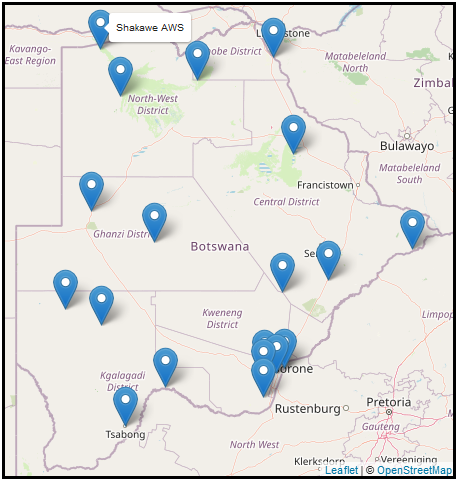
\includegraphics[width=1\linewidth, height=0.28\textheight]{fig/bw_AWS}
	\caption{Visualising Botswana AWS using  Algorithm \ref{TheMapper}.  
}
	\label{BW_Map}
\end{figure}

\noindent
%The WebSAPI   offers the possibility of selecting a station from a drop-down list  and other user inputs as shown in  Fig \ref{BW}. This eliminates possible typing errors that can be introduced by end users.%\\
 %\\
%\noindent
%The rvest package was used to simulate Web sessions and parse data in into a CSV format, although it can   be transformed to other   formats (i.e., excel). 
%The WebSAPI can access, extract, visualise and download (i.e., CSV format) the weather data at a fly. Depending on the arguments, if the script execution is successful, the entire dataset is saved into a chosen folder, with file names given by the end user.
The algorithms defined in section \ref{Scraper}   only scrape data from  one AWS at a time. These can be extend   by adding a functionality to specify  multiple AWSs   then   use a for loop function   to scrape  desired weather data as shown in Fig. \ref{SASSCAL_WebSAPIA}. 
\newpage
\noindent
%We show all the steps from requesting data, downloading data, through data processing, and analysis. 
%All these demonstrate the value that the SASSCAL WebSAPI provides through out the methodological pipeline and how it can aid researchers to apply SASSCAL weather data in their data driven projects.
\onecolumn
\begin{figure}
	\centering
	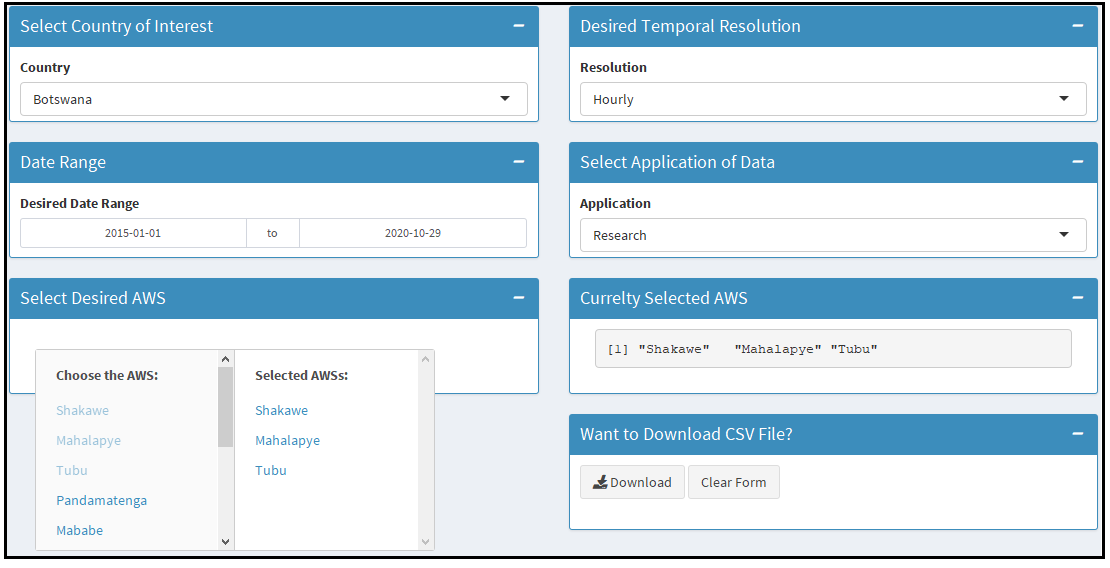
\includegraphics[width=1\linewidth]{fig/Selector}
	\caption{Screenshot of the SASSCAL WebSAPI for capturing user input when requesting weather data.  The GUI allows end users to select the geographical location of interest (i.e., Botswana), temporal resolution, the AWS of interest and the downloading of data. The functionality of multi-input selection of AWSs provides end users with a feedback mechanisms to notify about the selected AWS as seen on the tab titled ``Currently Selected AWS."
This is quite useful for a quick exploration of  geographic locations before downloading  data. 
}
	\label{SASSCAL_WebSAPI}
\end{figure}

\begin{figure}
	\centering
	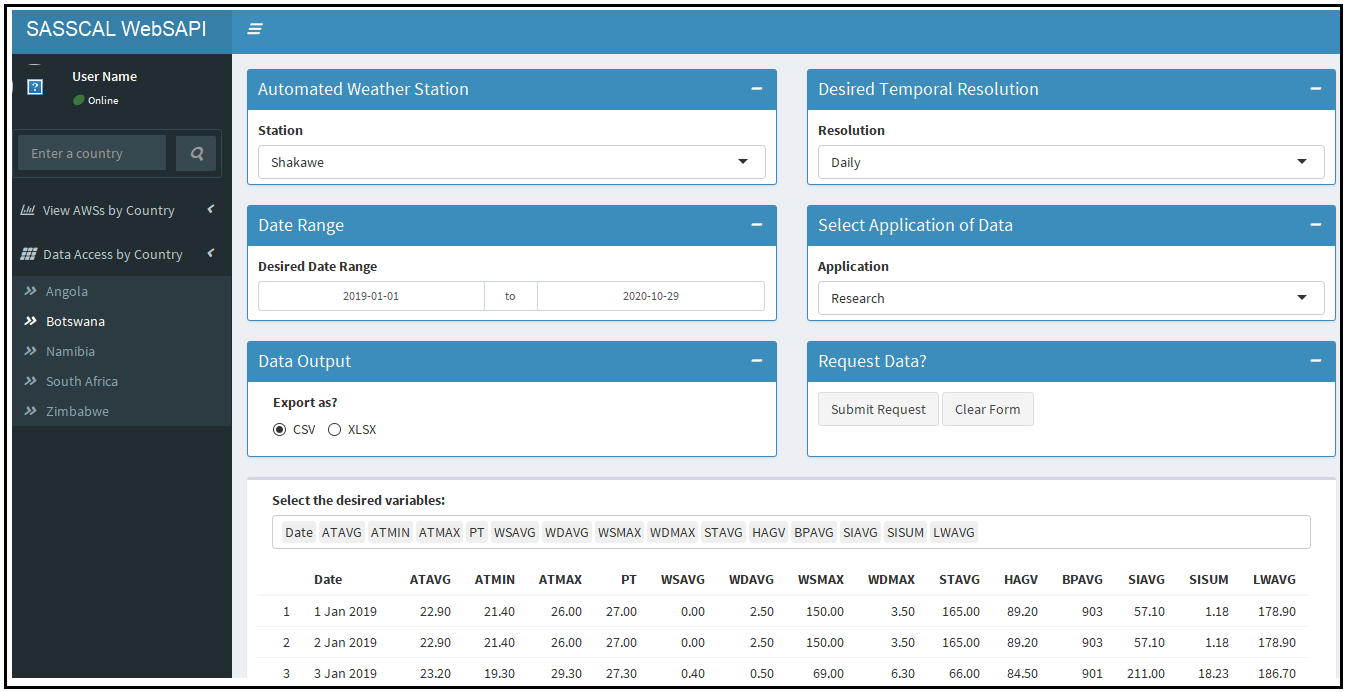
\includegraphics[width=1\linewidth, height=0.4\textheight]{fig/BW_Data}
	\caption{Screenshot of the SASSCAL WebSAPI's GUI for data request, visualisation and extraction of data. 
 In addition to selecting the desired AWS,    temporal resolution, and the date range, the SASSCAL WebSAPI's GUI allows end users to select the desired  variables.
}
	\label{SASSCAL_WebSAPIA}
\end{figure}


\twocolumn
\noindent



\section{\textbf{Discussions}}
%  1.Tells the main conclusion of the paper in one or two sentences.
%  2. Tells how the paper’s results contribute to answering the big questions posed in the Introduction.
%  3. Explains how (and why) this work agrees or disagrees with other, similar work.
%  4. Explains how the limitations of this study leave the big questions unanswered.
%  5. Tells how extensions of this paper’s results will be useful for answering the big questions.
\label{Discus}
\noindent
%Through this work, the SASSCAL WebSAPI was  developed with the aim of  supporting the  SASSCAL Weathernet platform.
In this work, a data driven template   was developed in the form of a WebSAPI to facilitate efficacious interaction with the outputs generated by the SASSCAL weathernet.
The SASSCAL WebSAPI implements   modularised  algorithms  to collect the SASSCAL weather data and generate high-quality data sets that can be used in data driven projects. 
Modularised scripts facilitate an efficient product design process that integrates any  efforts related to  idea generation, concept development, and, modification of existing systems and platforms to develop proper solutions.
%
This section %begins by presenting a usage example (just for illustrations) as a proof of concept of the generic pipeline deployed in this work. It also 
presents   discussions regarding the data quality, legal aspects, limitations and implications of   the  proposed  WebSAPI. 
%\\
%\\
%This work  aimed not at improving nor replacing the existing SASSCAL Weathernet but rather at supporting its services. 
%Without data, no data driven project can start  \cite{Abbott}.
%Through this work, a simple yet efficient platform was developed  to simplify  the problem of data accessibility.
%This philosophy of developing simple solutions for complex systems is also supported in Ref \cite{zungeru2018design}. 
%

%The  SASSCAL WebSAPI illustrated in Fig. \ref{BW} and Fig. \ref{SASSCAL_WebSAPIA} enables efficacious access to the SASSCAL weather data for further use in research. % applications.
%In particular, this work focused on answering the following  research question: ``How are the average maximum air temperatures distributed within the Okavango Delta region?"
%To give an answer to this question we refer to the data available on SASSCAL Weathernet. The website provide near to real time climatological data at intervals of 15 minutes, and the data is free to public through its dashboard.
%he SASSCAL Weathernet can be viewed as an online weather bulletin dashboard where the data collected through a network of SASSCAL AWSs can be consolidated and visualised. End users can then access the dashboard to view or extract weather data for use in their respective tasks.



%\subsection{\textbf{Usage Example}}
%\noindent
%The use of the SASSCAL data is motivated by  analysing the distribution of the  average  temperature data using    violin/Box-plots as motivated in  \cite{hintze1998violin}  (see Fig. \ref{BoxP2020}). 
% Previous studies \cite{kolawole2014ethno} indicate that the Okavango Delta is experiencing progressive increase regarding temperatures which ultimately lead to increase in potential evapo-transpiration \cite{moses2018effects}.  Another attempt was made in Ref \cite{thapelo2019machine} to use the SASSCAL data in predicting maximum and minimum temperatures at local level.
%For that reason, the Okavango Delta located in the north-west was selected as the study area. % The weather data was collected from the   Shakawe AWS located in the North West of the country. 
%The goal  was to investigate the variations (i.e., peaks) in the  data;  determining whether the temperature values were clustered around the median, the minimum or the maximum. 

%\begin{figure}[h]
%	\centering
%	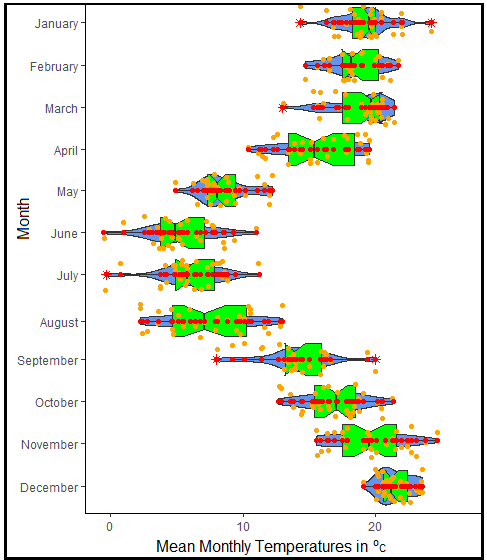
\includegraphics[width=0.8\linewidth]{fig/BoxP}
%	\caption{Violin/Box-plots showing  daily average air temperature distributions in \textcelsius\   for  Shakawe's AWS (January - December, 2015).
%	%	Data will be pulled for the selected SASSCAL AWS ID for the start and end year for each data source for a given time step.
%}
%	\label{BoxP2020}
%\end{figure}
%
%\noindent
%As it can be seen in Fig. \ref{BoxP2020}, daily mean temperatures (ATAVG) start increasing from September (commencement of summer), culminating around October-to-January when the sun is overhead at the tropic of Capricorn \cite{WeatherSilitshena}, then they decline gradually through March.  
%The ATAVG diminishes gradually from around April until reaching the lowest temperatures (in June and July) leading to a colder season (May to August) which concurs with reports in \cite{moses2017heat,Nkemelang2018}. 
%The mean temperature distributions at Shakawe AWS (for 2015) varies with respect to the months.
%The shapes of the distribution of June, July and September are extremely skinny on each end and wide in the middle. These indicate that the values of the daily mean temperature observations for these months are highly concentrated around the median. 
%
%\newpage
%\noindent
%The asterisks ({\color{red}*}) in Fig. \ref{BoxP2020} identify outlier temperatures (in January, March, July, and September), depicting observations outside the 99\% range of a normal distribution represented by   whiskers. The interesting thing about the presentation of data distributions using violin/Box-plots is that outlier temperature values can translate to heat wave observations which are of interest in health and agro-meteorology \cite{moses2018effects} and climatology. % (high temperatures lead to high evapo-transpiration \cite{moses2018effects}).
%\\
%\\
%The presentation of the weather outputs  in the form of  violin/Box-plots makes it easier for end users to compare the distributions  of weather data (in this case, average air temperatures) for a given location. This way, end users can have a visual picture of the patterns of weather variables of interest. 
%The SASSCAL WebSAPI is  efficient and inexpensive to use, yet with high potential to support efficiency in research.
%It avoids the time-consuming and repetitive human-engineered and error-prone manual steps of generating data sets.  
%This  will be  useful for any researcher; and other practitioners seeking to utilise the SASSCAL weather data in their data driven   projects.
%It should be noted as well that this work also contributes by  raising awareness of online SASSCAL scientific data which is open to public. 


\subsection{\textbf{Legality and Ethics of the SASSCAL WebSAPI}}
\noindent
%One of the main aim for this work was to  modify the SASSCAL WebSAPI by developing a  Robot Crawler and Scraper  targeted at automating the extraction and analysis of SASSCAL Weathernet at a fly (i.e., without locally storing the data). However, it was found necessary to analyse the data quality, legality and ethics of the proposed SASSCAL WebSAPI as presented below. 
%The  proposed Data Driven Framework   for web scraping and dashboard design takes into consideration the data quality, legality and ethics of the developed SASSCAL WebSAPI. % as presented below. %of scraping and use of   the SASSCAL  data. %Weathernet.
%\\
%\\
 The SASSCAL Weathernet data is checked for quality control as mentioned in Ref \cite{kaspar2015sasscal}.  This gives an ``assurance" that the SASSCAL WebSAPI will provide   quality data that would not mislead end users (i.e, researchers, or decision makers). However, users should note that due to occasional sensor faults, the correctness of  data values cannot be fully guaranteed as also indicated in the SASSCAL Weathernet\footnote{\url{http://www.sasscalWeathernet.org/imprint_we.php}}.  The declaration on SASSCAL data use  indicates that free use   is granted for non-commercial and educational purposes. %Commercial use can be granted based on requests submitted  to SASSCAL. 
 \\
\\
%However, there was need to reflect on whether the SASSCAL WebSAPI accessed the SASSCAL Weathernet in an authorized way.
Although there are no explicit restrictions on data scraping on the SASSCAL Weathernet,  it   is difficult to conclude that   SASSCAL encourages   end users to  automatically scrape and extract data using tailor made APIs. 
 This can be justified by the note ``For data requests regarding specific countries, stations, \emph{\underline{time periods}} or \emph{\underline{specific sensors}} please contact \url{oadc-datarequest@sasscal.org}" as shown in \footnote{\url{http://www.sasscalWeathernet.org/contact_we.php}}. It should be noted that the underlined aspects are the challenges proposed to be addressed through  this work. Thus, personal APIs that pro-grammatically extract the weather data by bypassing the designated SASSCAL Weathernet API can be seen as presenting  slight ethical dilemma for developers.
 

\subsection{\textbf{Challenges and Limitations}}
\noindent
%Thus, we concluded that we could go ahead and develop an R script that automatically scraped the pages and downloaded data. 
The main  hurdle  relates to identifying and integrating appropriate data driven technologies to facilitate flexible access and visualisation of  the SASSCAL weather data. In this regard, a couple of algorithms have been completed and tested to optimise the   task of web scraping.
However, the taks of  retrieving weather data was tested using relatively small dataset (94 instances). The small data set were chosen to ensure that the automatic scraping and retrieving of data does not likely damage or slow down the SASSCAL website's servers. 
This toolkit is built on top of the SASSCAL Weathernet. Thus, changes in  structural representation of  SASSCAL Weathernet  implies modifying  the    WebSAPI.  

\subsection{\textbf{Lesson Learnt}}
\noindent
There is no free lunch in  problem solution. The process of web scraping and dashboard     design is iterative and evolutionary. The integration of R, flexdashboard and Shiny allows the development and  deployment of interactive apps. 
%The RMakrdown, coupled with  Shiny and flexdashboard are becoming an increasingly popular tool for highly customised data visualisations  and modern interactive  dashboards.  
However, before starting a web scraping based  data driven project, developers   should   start by analysing  associated legality and ethics  \cite{mason1986four,krotov2020tutorial}   to avoid  possible bottlenecks.

\newpage
\noindent
%The   data used for demonstrations  was limited to one year, and collected from one AWS. Hence, the analysis cannot generalise for a larger spatial geographical region. 
% The SASSCAL WebSAPI currently allows the extraction of data from one station at time; using some  user inputs like station name as seen in   Fig. \ref{SASSCAL_WebSAPIA}.
 %There is no capability to extract and analyse data from multiple AWSs at a go.
\subsection{\textbf{Contribution and Implications}}
\noindent
%We were able to quickly adapt to changing circumstances, interfaces and
%user requests, while still maintaining a highly automated, cost-effective and scalable platform.
 %\\
 %\\
The contribution of this work is rather pragmatic than theoratical. 
%The approach deployed herein is reproducible and hence  support reuse of modulirised algorithms \cite{seol2007design}.
%The WebSAPI takes into consideration: data scraping, data visualisation and sharing of outputs. 
The     WebSAPI is flexible and reproducible,
with potential to be scaled up (expanded) to address other functionalities related to the use of   SASSCAL weather data. 
Reproducibility  is an important aspect in open science research  and API development. 
This helps to reduce time taken for data collection, development and testing since the independent components (algorithms) have been already tried and tested.
This  approach   has   potential to  catalyse the development of   packages  from existing platforms to meet   the end user requirements.
%To the best knowledge of the authors, the data was used for research, which is a legitimate. %, non-fraudulent task that does not even infringe any IP rights.
%Therefore, this work's outputs   would not somehow diminish the SASSCAL website’s data. 
%Moreover, the aggregated weather data     at local levels (i.e., on monthly basis) can expose certain patterns of air temperatures at localised stations. 
It should be noted that neither the BDMS nor BIUST have an API to disseminate weather information. 
This WebSAPI is still   under development, yet with potential to be adapted and incorporated to portals of weather service providers (BIUST, BDMS, SASSCAL, and WASCAL)   to bridge gaps of weather and climate data access.

	\section{\textbf{Conclusion}}
	\label{Conclu}
	\noindent
	% short summary of the findings and its meaning for the broad research area.
%	The SASSCAL data is growing at a fast rate, and tangled within it are new opportunities in environmental data science \cite{GIBERT20183}.
\subsection{Summary}
\noindent
Developing and implementing a data driven platform to serve end users is a challenging task that requires input from multidisciplinary stake holders. This work integrated web scraping \cite{WebSrapping}, data wrangling and dashboard techniques   to develop a lightweight SASSCAL WebSAPI.
In  comparison  to  previous web scraping literature,  this work   takes  into consideration that data driven outputs need to be disseminated to end users. In this case, a dashboard proto-type was developed in RMarkdown to facilitate reproducibility. The WebSAPI is expected to create new channels to extend services of the SASSCAL Weathernet.
By enabling efficacious and efficient data access, the SASSCAL WebSAPI has potential to increase   productivity and quality of data driven  projects that make use of  SASSCAL weather data.
%All these could enable end users to quickly: query weather data banks; explore 	several weather data sets and   summarise their statistics; build predictive models \cite{Abbott}; extract hidden patterns; and make well informed decisions when generating solutions to problems pressing  societies. Lastly, 

\subsection{\textbf{Future Work}}
\noindent
The  SASSCAL WebSAPI  should be seen  not as a replacement but rather  a  complementary
toolkit to   SASSCAL. It does not cover all the tasks related to ``weather data science", but it provide the end-user community with the opportunity to reproduce it and  develop in-depth product development skills to ultimately add more functionalities to a related API. 
In terms of extending this work, more end-user driven functionalities will be added to this API to enable  data driven operations and services like investigating strategies for imputation of missing  data, and  modelling. % using the historical   weather data.
  %Future objectives include implementation of a Robot Crawler and Scraper (RCS) to  extract  data   from various online weather data banks. 

\subsection{\textbf{Recommendations}}
\noindent
The collaboration with the concerned   stakeholders (i.e, SASSCAL, BDMS, BIUST), including end users (researcher, students, and  farmers) could catalyse the development and deployment process.
  This will surely enhance operational productivity while  maximizing  utilization of these amazing open-source technologies.
Efforts from this work are  likely to spawn new projects and collaboration that will better inform citizens and continue to help them to make use of the generated data, and  contribute to the open-data community.
%The SASSCAL WebSAPI aims to   create new channels  to  extend  services of the SASSCAL Weathernet.  The toolkit facilitates end users to efficaciously access  and extract  weather data from the  SASSCAL Weathernet. 	  
%	 	Web scraping and data wrangling techniques  were used to automatically generate weather data sets. A Shiny dashboard was developed to visualise and disseminate outputs to end users. 	 	The toolkit  increases productivity, efficiency and quality of  projects that make use of  data from SASSCAL's AWSs. 
%	 	This  toolkit is  valuable  for researchers and analysts who seek to integrate the SASSCAL weather data in their   projects. 
%	 	The toolkit  was  deployed  in a case study to present new statistical analyses of  extreme temperatures in the Okavango Delta.  
%	 This toolkit is expected to catalyse many other research  projects like  in the analysis of heat waves, soil erosivity and erosivity density). 
	 

%\section{Recommendations}
%\label{Reco}
%\noindent
%This work motivates the use of  open source technologies to access or visualise data from online climatic data banks.  
%The SASSCAL WebSAPI can be implemented to  bridge gaps  of climate data access at local %to regional
%levels. It should be noted that neither the BDMS nor  BIUST have an API for dissemination of weather and climate information.    Therefore, the SASSCAL WebSAPI  can be adapted and incorporated to portals of weather service providers (like BIUST and SASSCAL) to facilitate open access to weather data.
%All these could enable end users to  quickly explore 	several weather data sets and  summarise their statistics to make well informed decisions regarding their data source and sample sizes.

%\section{Future Directions}
%\label{Futuro}
%\noindent
%More end user-driven functionalities will be added to this API to: (1) improve the user interface to support access mechanisms to the SASSCAL Weathernet; (2)  monitor the research data be accessed; and (3)  investigate strategies for imputation of missing weather data using the historical  SASSCAL weather data. 
%Given that the Weathernet portal may also change, future directions can be focusing on implementing a sustainable  way of identifying and extracting
%  data   from different web sources. 
%However, designing the Robot Crawler and Scraper clearly necessitates collaboration with the SASSCAL organisation to make all the steps smoother.
%This work  will continue to motivate and encourage the use of weather and climate data that is normally archived and left under utilised, especially in developing regions. 

 


\section*{\textbf{Acknowledgements}}
	\noindent
BIUST: for the partial financial support (with reference number: S-00086); and SASSCAL  for availing the  data.  

\newpage

\section*{\textbf{Author roles}}
\noindent
Thapelo T.S: Conceptualization, Methodology, Resources, Application Development, Writing (Original Draft Preparation; Review and Editing);
Namoshe M:  Conceptualization, Resources, Formal Analysis, Review and Editing;
 Matsebe O: Conceptualization, Resources, Formal Analysis, Review and  Editing;
 Motshegwa T: Resources, Formal Analysis, Review and Editing; 
Bopape MJM: Resources, Formal Analysis, Review and Editing.

\section*{\textbf{Competing Interests}}
None
\section*{\textbf{Reproducibility}}
\noindent
This  R based toolkit  is still under development. 
Parallel to this manuscript is a reproducible tutorial in RMarkdown, integrating Shiny  and Flaxdashboard for visualisation and dissemination of outputs. % of outputs based on the same data. 
The tutorial and code is available on \url{https://github.com/EL-Grande/SASSACL-WebSAPI} and the data is available online \ref{Weatherneto}. %github: https://github.com/cocomice/EDSS_dep_framework
%\newpage



%%%%%%%%%%%%%%%%%%%%%%%%%%%%%%%%%%%%%%%%%%%%%%%%%%%%%%%%%%%%%%%%%%%%%%%%%%%%%%%%

\bibliographystyle{ieeetr}
\bibliography{MiBib}

\end{document}
